%==============================================================================
% locality-approach.tex
%==============================================================================

\chapter{Approach}
\label{chap:locality-approach}

Before starting with the implementation of the new scheduler, we
implement a synthetic multi-threaded locality-aware benchmark called
\emph{Cache Stress Test}. This benchmark serves as a proof of concept
for our plan to introduce locality-aware intervals: If a
multi-threaded benchmark with best possible locality has better
performance and fewer last-level cache misses than the same benchmark
with another or no specific locality, we should be able to see the
same effect when porting the benchmark to a locality-aware
implementation of intervals. Hence, we know whether it makes sense to
design a locality-aware intervals scheduler.

We wrote our benchmark for the Intel Nehalem system described in
Appendix \ref{sec:experimental-setup-mafushi}. The system has 2
processors with 4 cores each. Every core has its separate level 1 and
2 caches, but the per-processor 8 MB level 3 cache is shared between
all cores of the same processor. The methodology we use to run the
benchmarks and measure their results is presented in Section
\ref{sec:locality-performance-methodology}.

\emph{Cache Stress Test} first randomly initializes two integer arrays
of size \numprint{2097144}, i.e. the size of each array is about 8
MB. This is equal to the size of the last level cache per
processor. Then the benchmark creates 8 \emph{Cache Stress} threads
for each core with their affinity set to this specific core. Overall,
we create 64 threads, bound to the 8 cores in groups of 8 threads. To
bind threads to a specific core, we use the affinity library
introduced in Section \ref{sec:locality-implementation-core-affinity}.

One half of the threads operate on the elements of the first array and
the other half operate on the elements of the second array. Each
thread adds and multiplies all the elements of its respective array
100 times.

We implement several different variants of the \emph{Cache Stress
  Test}, each having different locality properties:

\begin{description}
\item[Best Locality:] All the threads working on the first array have
  affinity for a core on the first processor and all threads working
  on the second array have affinity for a core on the second
  processor.
\item[Ignorant Locality:] The threads are not bound to any specific
  core, i.e. they are \emph{ignorant} of their locality.
\item[Random Locality:] The affinity of the threads is set to a
  \emph{random} core.
\item[Worst Locality:] Half the threads with affinity for a core on
  the first processor work on the first array, and the other half
  works on the second array and vice versa.
\end{description}

Figure \ref{fig:locality-approach-cache-stress-test-mafushi}
illustrates the core affinities of the threads for the \emph{best} and
\emph{worst locality}.

\begin{figure}[!ht]
  \centering
  \subfloat[Best Locality]{
    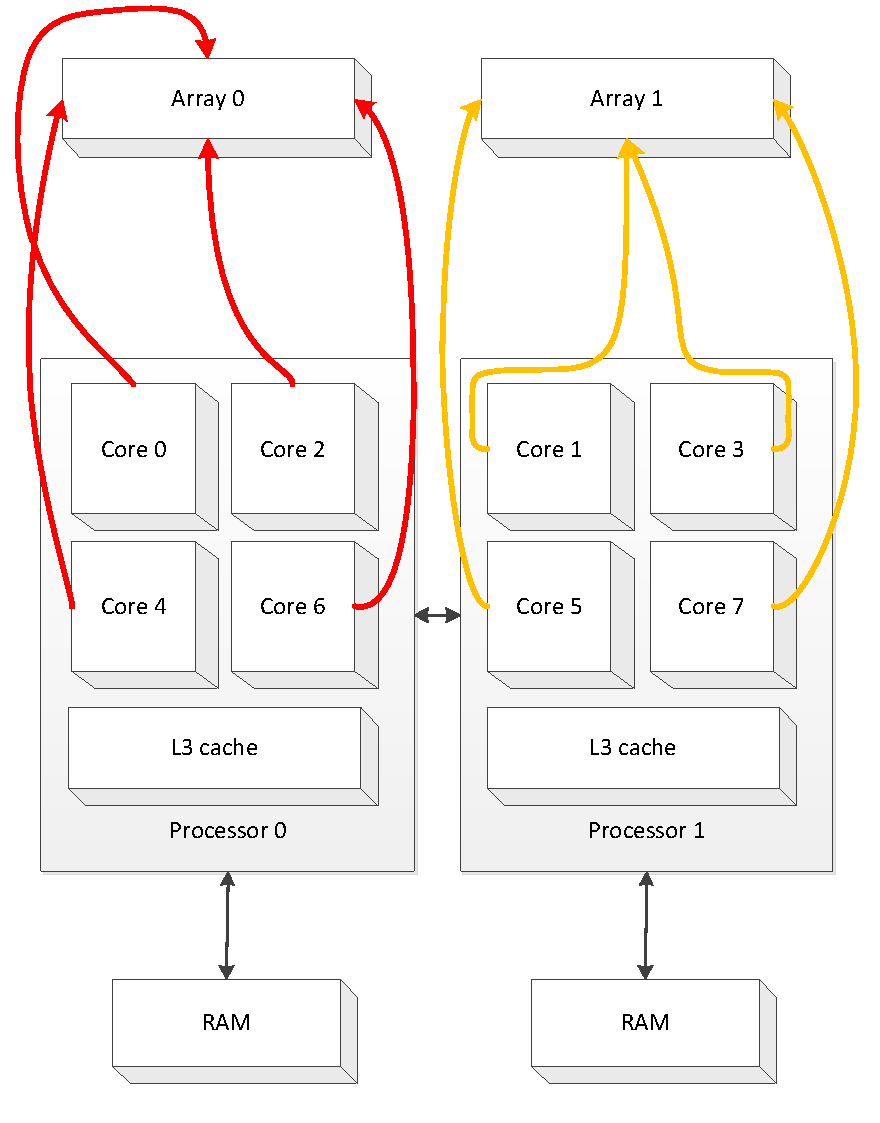
\includegraphics[width=0.5\linewidth]{locality-approach/cache-stress-test-mafushi-best}
    \label{fig:locality-approach-cache-stress-mafushi-best}
  }
  \subfloat[Worst Locality]{
    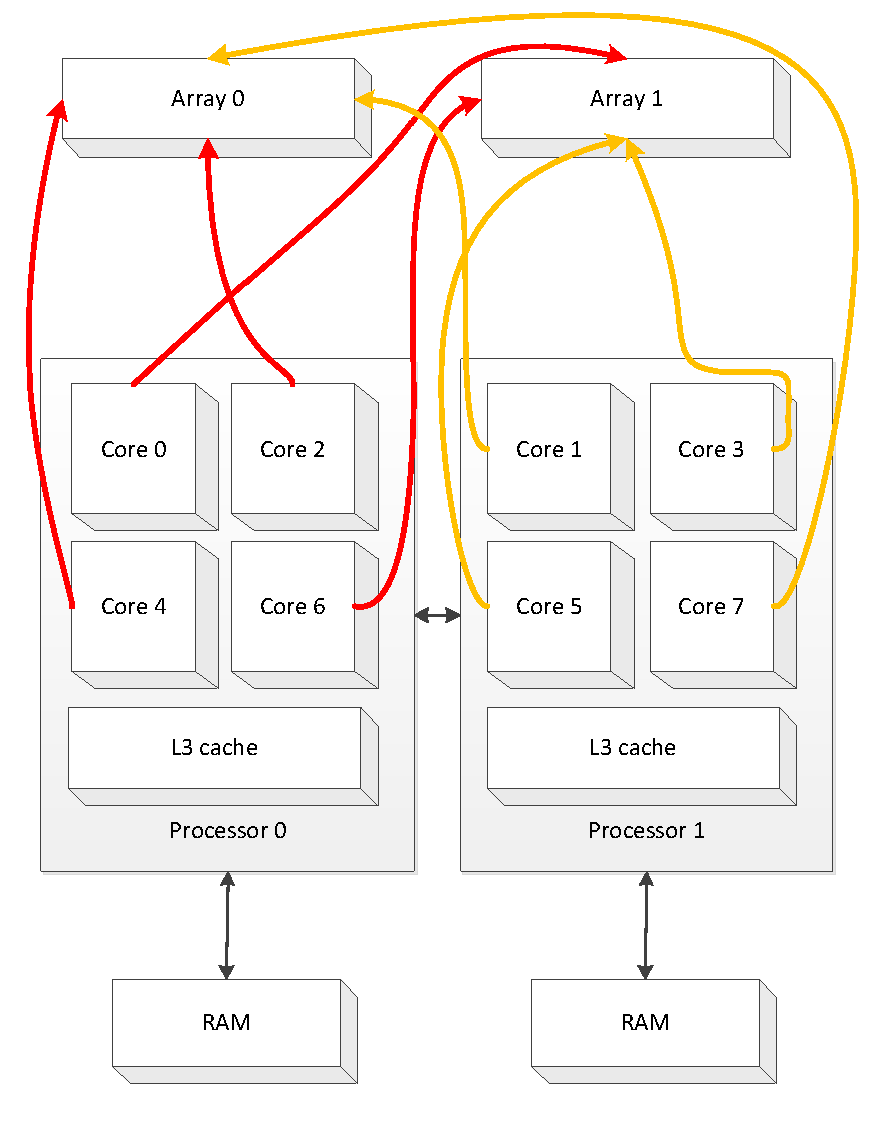
\includegraphics[width=0.5\linewidth]{locality-approach/cache-stress-test-mafushi-worst}
    \label{fig:locality-approach-cache-stress-mafushi-worst}
  }
  \caption{Multi-threaded \emph{Cache Stress Test} with \emph{best}
    and \emph{worst locality}}
  \label{fig:locality-approach-cache-stress-test-mafushi}
\end{figure}

As the name already gives away, the main idea behind the \emph{Cache
  Stress Test} benchmark is to stress the cache and provoke cache
prefetching and contention.

When we are using the \emph{best locality} benchmark, we move all
sharing threads onto the same processor which will perform prefetching
of the array elements for each other. That is, they help to obtain and
maintain the frequently used array elements in the local L3 cache.

The exact opposite happens in the other variants: Threads compete for
the L3 caches and overwrite each other's entries. Instead of reading
from the processor's local cache, threads either have to read from the
other processor's cache or the memory subsystem. Reading from those
places is much more expensive than reading from the local L3
cache. Table \ref{tab:locality-introduction-memory-access-times} cites
\textcite{Levinthal2009} and gives rough approximations for the memory
access times on our test system. The latencies depend on the core and
uncore frequencies, memory speeds, BIOS settings, number of DIMMs, and
so forth.

\begin{table}[htb]
  \centering
  \begin{tabular}{ll}
    \toprule
    Data Source & Latency \\\midrule
    L3 cache hit, line unshared & $\sim 40$ cycles\\
    L3 cache hit, shared line in another core\hspace{0.5cm} & $\sim 65$ cycles \\
    L3 cache hit, modified in another core & $\sim 75$ cycles \\
    Remote L3 cache & $\sim 100 - 300$ cycles \\
    Local DRAM & $\sim 60$ ns \\
    Remote DRAM & $\sim 100$ ns \\\bottomrule
  \end{tabular}
  \caption{Memory access times on the Intel Nehalem processor}
  \label{tab:locality-introduction-memory-access-times}
\end{table}

Table \ref{tab:locality-approach-cache-stress-test} shows the
execution times and the speedups over the sequential algorithm for the
different locality implementations. As expected, the implementation
with \emph{best locality} is the fastest and provides the largest
speedup.

\begin{table}[htb]
  \centering
  \begin{tabular}{ln{2}{3}n{1}{2}}
    \toprule
    & {Runtime (in seconds)} & {Speedup (over sequential)} \\\midrule
    \emph{Best Locality} & 3.327 & 7.69 \\
    \emph{Ignorant Locality} & 3.985 & 6.42 \\
    \emph{Random Locality} & 5.175 & 5.83 \\
    \emph{Worst Locality} & 4.389 & 4.94 \\
    \emph{Sequential Implementation}\hspace{0.5cm} & 25.571 & 1 \\\bottomrule
  \end{tabular}
  \caption[Multi-threaded \emph{Cache Stress Test} execution times]{Multi-threaded \emph{Cache Stress Test} execution times and speedups over the sequential implementation}
  \label{tab:locality-approach-cache-stress-test}
\end{table}

Figure \ref{fig:locality-approach-cache-stress-test} illustrates the
execution times normalized to that of the \emph{best locality}
implementation. The \emph{best locality} implementation shows a
significant speedup over the other locality benchmarks of
$1.2\times$ -- $1.55\times$.

\begin{figure}[!ht]
  \centering
  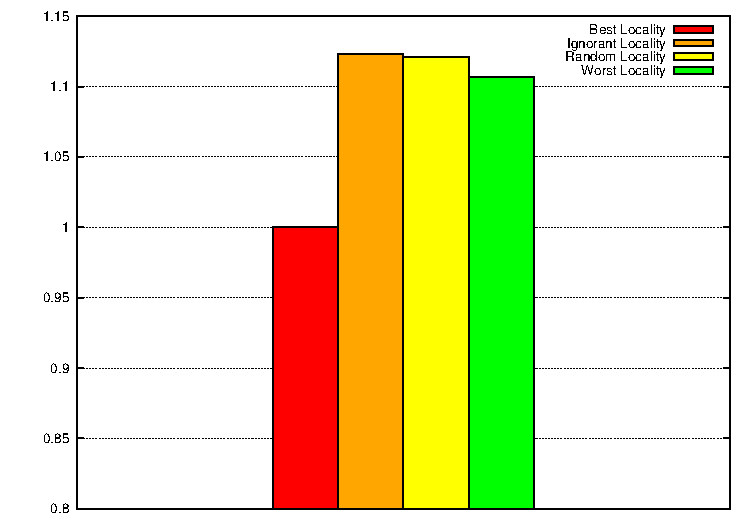
\includegraphics[width=0.8\linewidth]{locality-approach/cache-stress-test}
  \caption[Multi-threaded \emph{Cache Stress Test}
  execution times]{Multi-threaded \emph{Cache Stress Test} with execution
    times normalized to \emph{best locality}}
  \label{fig:locality-approach-cache-stress-test}
\end{figure}

Table \ref{tab:locality-approach-cache-stress-test-cache-hits-misses}
lists the number of L3 cache read hits and misses. In Figure
\ref{fig:locality-approach-cache-stress-test} they are shown
normalized to the measurements of the \emph{best locality}
implementation. 

Compared to the other benchmarks, the \emph{best locality} benchmark
has between $1.5\times$ and $1.8\times$ more L3 cache read hits, and
between $3.6\times$ and $4.5\times$ fewer L3 cache read misses.

\begin{table}[htb]
  \centering
  \begin{tabular}{ln{4}{0}n{4}{0}}
    \toprule
    & {L3 Cache Read Hits}  & {L3 Cache Read Misses} \\\midrule
    \emph{Best Locality}\hspace{1cm} & 2577 & 219\\
    \emph{Ignorant Locality} & 1674 & 800 \\
    \emph{Random Locality} & 1646 & 894 \\
    \emph{Worst Locality} & 1387 & 1005 \\\bottomrule
  \end{tabular}
  \caption[Multi-threaded \emph{Cache Stress Test} L3 cache read hits and misses]{Multi-threaded \emph{Cache Stress Test} L3 cache read hits and misses (rounded to the nearest million)}
  \label{tab:locality-approach-cache-stress-test-cache-hits-misses}
\end{table}

\begin{figure}[!ht]
  \centering
  \subfloat[L3 Cache Read Hits]{
    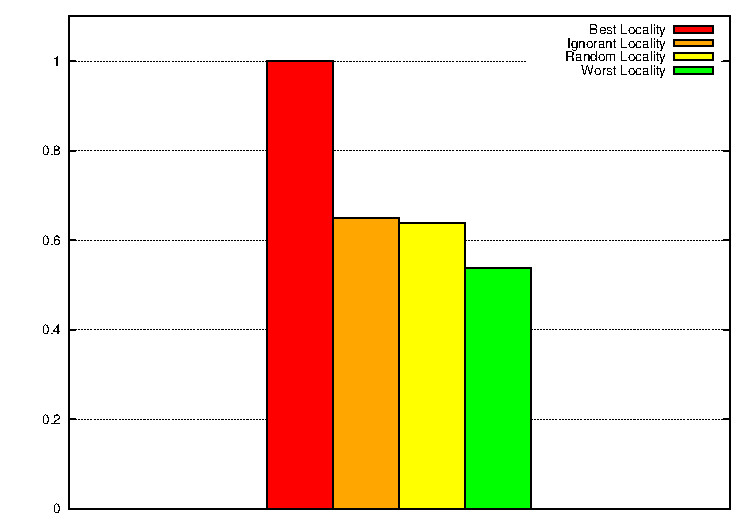
\includegraphics[width=0.5\linewidth]{locality-approach/cache-stress-test-cache-hits}
    \label{fig:locality-approach-cache-stress-test-cache-hits}
  }
  \subfloat[L3 Cache Read Misses]{
    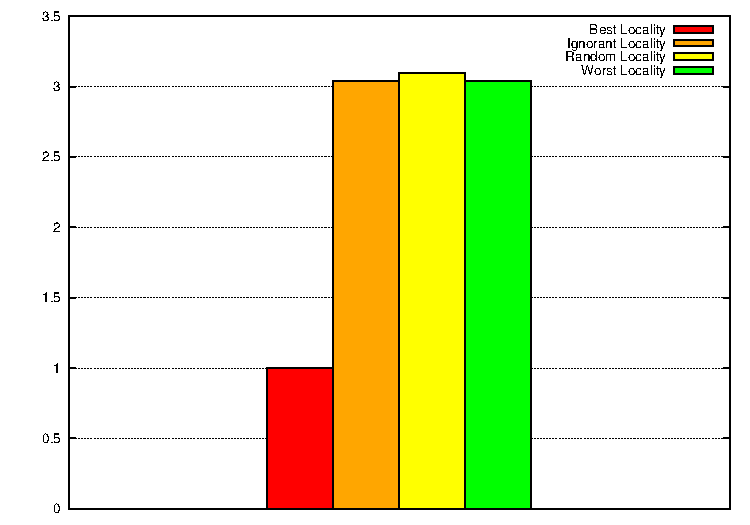
\includegraphics[width=0.5\linewidth]{locality-approach/cache-stress-test-cache-misses}
    \label{fig:locality-approach-cache-stress-test-cache-misses}
  }
  \caption[Multi-threaded \emph{Cache Stress Test} L3 cache read hits
  and misses]{Multi-threaded \emph{Cache Stress Test} with L3 cache
    read hits and misses normalized to \emph{best locality}}
  \label{fig:locality-approach-cache-stress-test-cache}
\end{figure}

Our experiments confirmed the hypothesis that the locality of threads
matters. Thus, we decided to rewrite the intervals scheduler to
support locality hints provided by the programmer. Chapter
\ref{chap:locality-implementation} describes the implementation of the
locality-aware scheduler for intervals, LASSI. In Chapter
\ref{chap:locality-performance} we evaluate the performance of LASSI
with a variety of benchmarks.


%%% Local Variables: 
%%% mode: latex
%%% TeX-master: "thesis"
%%% End: 